\section{Разработка TLA+ спецификации алгоритма Raft}

В рамках технологической части была разработана формальная
спецификация алгоритма консенсуса Raft на языке TLA+. Спецификация
используется для описания поведения кластера в терминах состояний,
переходов и сообщений, а также служит основой для последующей
модельной проверки и интеграции с системой верификации соответствия
спецификации и программной реализации.

\subsection{Формальная спецификация алгоритма}

В данном подразделе рассматривается разработанная TLA+ спецификация
алгоритма консенсуса Raft. Описание организовано по основным элементам
спецификации: константам, переменным, вспомогательным функциям,
действиям, оператору переходов и проверяемым инвариантам. Полный текст
спецификации можно найти в \cite{abeille} в папке \texttt{spec}.

На рис.~\ref{fig:tla-01} приведены константы спецификации. Константы в
TLA+ представляют собой неизменяемые в пределах спецификации значения.
Они определяются в начале модуля и используются для задания параметров
конфигурации, которые определяют поведение модели, но не изменяются в
ходе её выполнения. Конкретные значения констант задаются при проверке
модели.

\begin{figure}
  \centering
  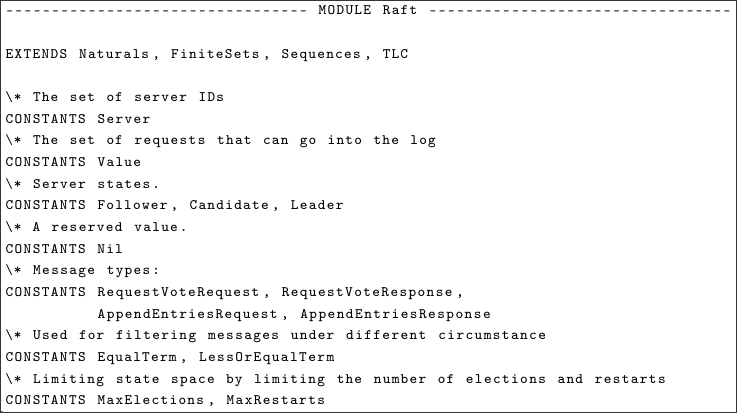
\includegraphics[scale=0.45]{inc/tla-01.png}
  \caption{Описание констант спецификации}
  \label{fig:tla-01}
\end{figure}

На рис.~\ref{fig:tla-01} задаётся основная среда протокола: множество
серверов, множество значений, роли узлов, типы сообщений, специальные
маркеры и ограничения, введённые для сокращения пространства
состояний.

$EXTENDS$ определяет, какие стандартные модули TLA+ подключены в
спецификации:

\begin{itemize}
    \item $Naturals$ --- для работы с натуральными числами и базовыми
    арифметическими операциями;
    \item $FiniteSets$ --- для работы с конечными множествами,
    например для вычисления мощности множества;
    \item $Sequences$ --- для работы с последовательностями, включая
    операции $Len$, $Append$, $SubSeq$ и другие;
    \item $TLC$ --- для использования вспомогательных средств
    моделирования и отладки, например операторов $Print$ и
    $Permutations$.
\end{itemize}

$CONSTANTS\ Server$ задаёт множество идентификаторов серверов. В TLA+
это стандартный способ описания системы, состоящей из конечного набора
узлов, например $\{s1, s2, s3\}$.

$CONSTANTS\ Value$ задаёт множество возможных значений, то есть
пользовательских запросов, которые могут добавляться в журналы
серверов.

$CONSTANTS\ Follower,\ Candidate,\ Leader$ обозначают три возможных
состояния сервера в алгоритме Raft: последователь, кандидат и лидер.

$CONSTANTS\ Nil$ определяет специальное пустое значение, используемое в
случаях, когда необходимо явно задать отсутствие некоторого объекта или
ссылки.

Блок констант $RequestVoteRequest$, $RequestVoteResponse$,
$AppendEntriesRequest$, $AppendEntriesResponse$ задаёт четыре типа
сообщений, используемых в Raft: запрос голосования, ответ на запрос
голосования, запрос репликации записей и ответ на него.

Константы $EqualTerm$ и $LessOrEqualTerm$ задают два режима проверки
срока, используемые при обработке сообщений: точное совпадение срока
или отношение <<меньше либо равно>>.

Константы $MaxElections$ и $MaxRestarts$ задают ограничения на число
выборов лидера и перезапусков узлов. Они вводятся для ограничения
пространства состояний модели при её практической проверке.

Глобальная переменная, разделяемая всеми серверами, в спецификации
только одна --- $messages$. Она представляет собой мультимножество
сообщений, циркулирующих в системе. В коде это задаётся как функция
вида $Message \rightarrow Nat$, где значением является число копий
данного сообщения, находящихся в канале.

На рис.~\ref{fig:tla-02} приведены вспомогательные переменные модели.

\begin{figure}
  \centering
  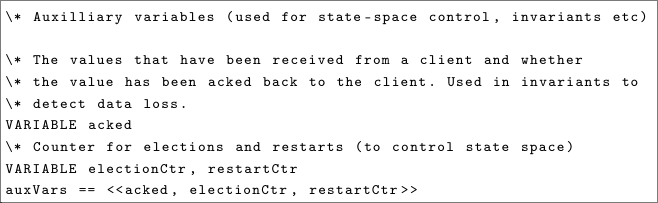
\includegraphics[scale=0.6]{inc/tla-02.png}
  \caption{Описание вспомогательных переменных}
  \label{fig:tla-02}
\end{figure}

$acked$ представляет собой отображение
$Value \rightarrow \{Nil, FALSE, TRUE\}$. Оно показывает, было ли
значение подтверждено сервером обратно клиенту. Если
$acked[v] = FALSE$, то запрос уже поступил, но ещё не подтверждён;
если $acked[v] = TRUE$, то запрос подтверждён; значение $Nil$
означает, что данный запрос ещё не предлагался. Переменная используется
при формулировке инвариантов, связанных с сохранностью данных.

$electionCtr$ и $restartCtr$ являются счётчиками, ограничивающими
пространство состояний. Они отражают число выборов лидера и
перезапусков узлов соответственно, а их верхние границы задаются
константами $MaxElections$ и $MaxRestarts$.

Все переменные, приведённые на рис.~\ref{fig:tla-03}, определены для
каждого сервера, то есть представляют собой функции от идентификатора
сервера из множества $Server$.

\begin{figure}
  \centering
  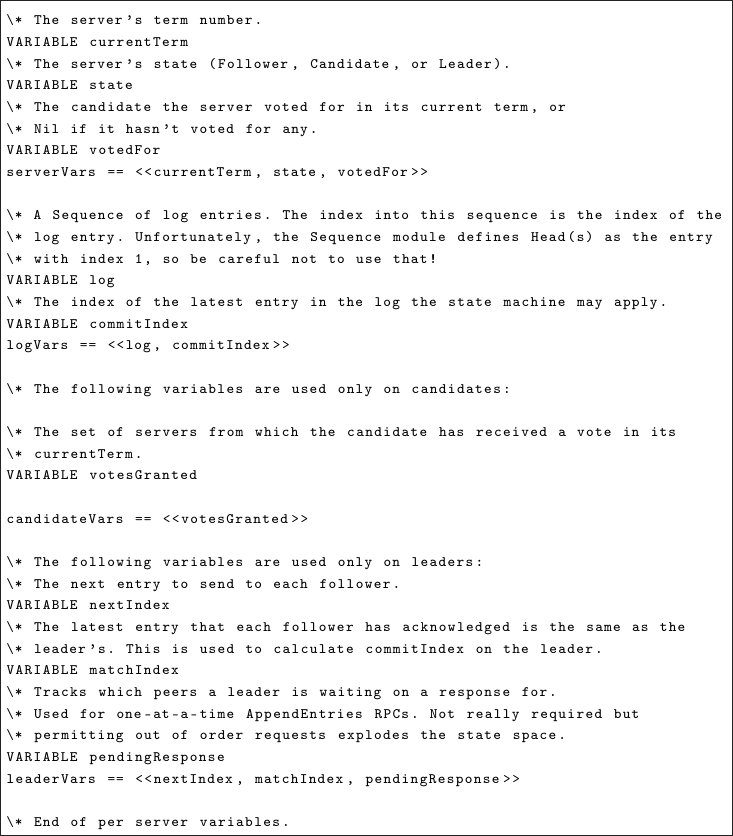
\includegraphics[scale=0.6]{inc/tla-03.png}
  \caption{Переменные сервера}
  \label{fig:tla-03}
\end{figure}

$currentTerm$ хранит для каждого сервера номер текущего срока.

$state$ задаёт текущее состояние сервера: $Follower$, $Candidate$ или
$Leader$.

$votedFor$ хранит для каждого сервера идентификатор узла, которому был
отдан голос в текущем сроке, либо $Nil$, если голос ещё не отдан.
Указанные переменные объединены в $serverVars$ для удобства обращения,
например при использовании в операторах справедливости.

$log$ представляет собой функцию от $Server$, сопоставляющую каждому
серверу последовательность записей журнала. Каждая запись содержит,
как правило, срок и значение.

$commitIndex$ показывает, до какого индекса журнал считается
зафиксированным, то есть готовым к применению к машине состояний.

$votesGranted$ хранит для сервера, находящегося в состоянии
$Candidate$, множество серверов, от которых получены голоса в текущем
сроке.

$nextIndex$ задаёт для каждого лидера и каждого сервера индекс, с
которого лидер должен отправлять записи при репликации. Если
$nextIndex[i][j] = k$, то лидер $i$ должен отправить серверу $j$
записи, начиная с индекса $k$ в собственном журнале.

$matchIndex$ задаёт для лидера $i$ и сервера $j$ максимальный индекс,
до которого журнал сервера $j$ гарантированно совпадает с журналом
лидера.

$pendingResponse$ задаёт для лидера $i$ и сервера $j$ булево значение,
показывающее, ожидает ли лидер ответа на ранее отправленный вызов
$AppendEntries$. Если $pendingResponse[i][j] = TRUE$, то повторная
отправка нового запроса тому же серверу не допускается. Это ограничение
введено для того, чтобы избежать чрезмерного роста пространства
состояний.

Реализация вспомогательных функций приведена на
рис.~\ref{fig:tla-04}. Эти функции не определяют собственные переходы
системы, а используются при инициализации, отправке сообщений и
обработке действий.

\begin{figure}
  \centering
  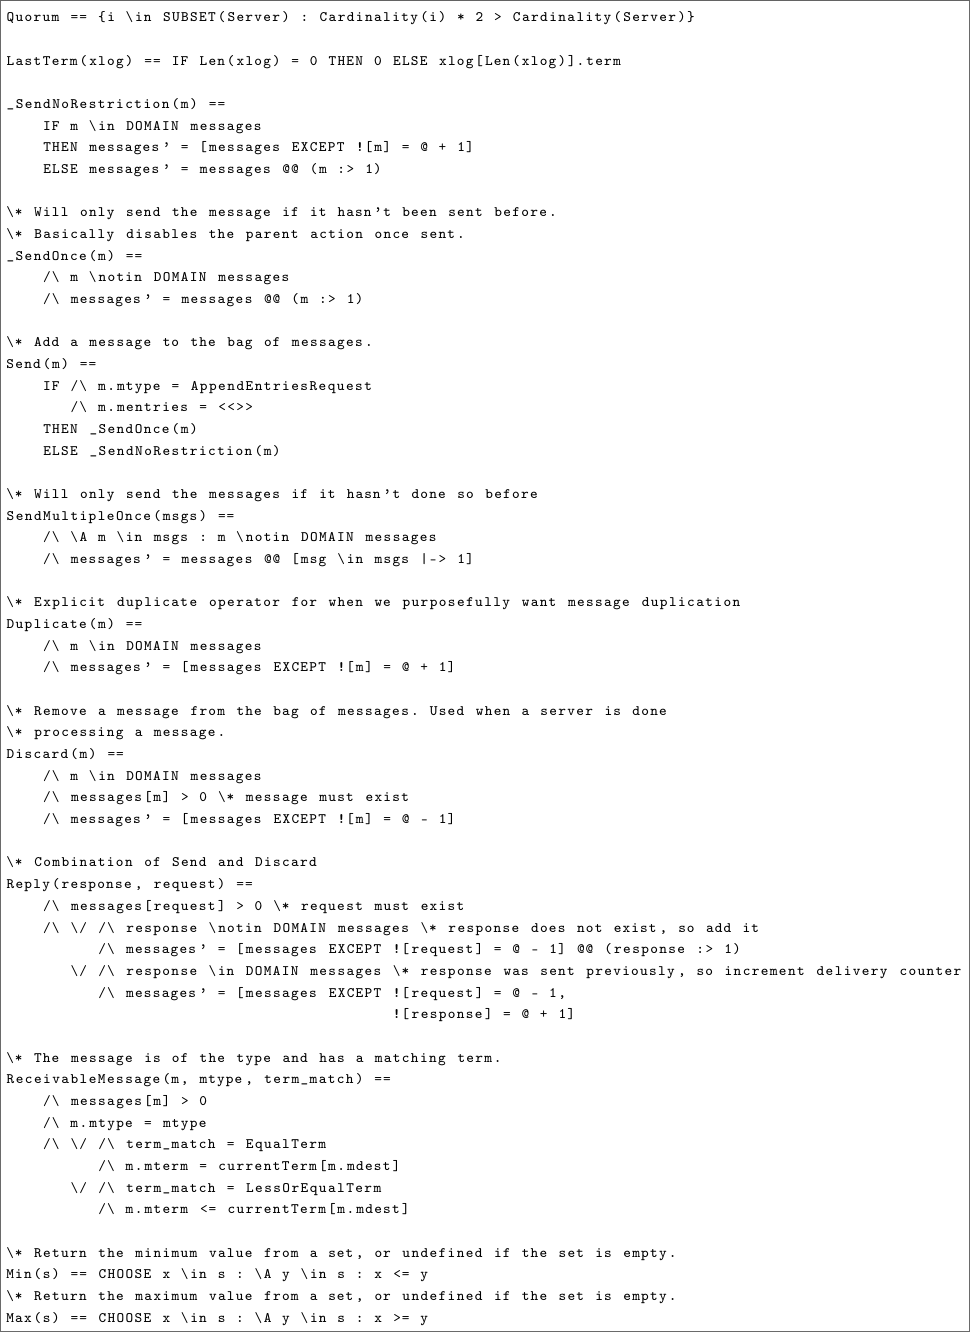
\includegraphics[scale=0.5]{inc/tla-04.png}
  \caption{Вспомогательные функции}
  \label{fig:tla-04}
\end{figure}

$Quorum$ задаёт множество всех подмножеств серверов, образующих
мажоритарный кворум. Если размер кластера равен $N$, то в кворум
входит строго более $N/2$ узлов. Любые два таких кворума пересекаются
хотя бы по одному узлу.

$LastTerm(xlog)$ возвращает срок последней записи журнала, либо $0$,
если журнал пуст.

$\_SendNoRestriction(m)$ добавляет сообщение $m$ в мультимножество
$messages$, увеличивая число его копий. Если сообщение уже существует,
его счётчик увеличивается, иначе создаётся новая запись.

$\_SendOnce(m)$ отправляет сообщение $m$ только в том случае, если оно
ещё отсутствует в $messages$. Эта функция используется там, где
повторная отправка могла бы существенно увеличить пространство
состояний, например для пустых вызовов $AppendEntries$.

$Send(m)$ является общей операцией отправки сообщения. Для пустого
$AppendEntriesRequest$ используется правило однократной отправки, в
остальных случаях допускается добавление сообщения без такого
ограничения.

$SendMultipleOnce(msgs)$ позволяет отправить набор сообщений за один
шаг, если ни одно из них ранее не присутствовало в $messages$. Обычно
эта функция используется для рассылки запросов голосования всем
остальным серверам.

$Duplicate(m)$ моделирует возможное дублирование сообщения в сети за
счёт увеличения его счётчика.

$Discard(m)$ удаляет одно вхождение сообщения из мультимножества
$messages$. Если копий несколько, счётчик уменьшается на единицу.

$Reply(response, request)$ объединяет в одном действии удаление
входящего сообщения $request$ и отправку ответа $response$.

$Min$ и $Max$ используются для выбора минимального и максимального
элемента множества.

На рис.~\ref{fig:tla-05} приведён оператор инициализации модели,
задающий полное начальное состояние кластера Raft: все серверы
находятся в состоянии $Follower$, имеют начальный срок $1$, пустые
журналы, отсутствующие сообщения в сети и нулевые значения счётчиков.

\begin{figure}
  \centering
  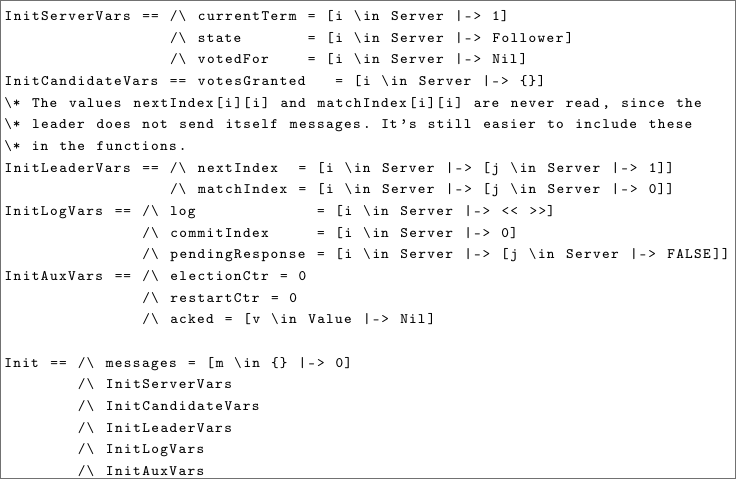
\includegraphics[scale=0.6]{inc/tla-05.png}
  \caption{Инициализация модели}
  \label{fig:tla-05}
\end{figure}

Важно отметить, что все переменные, кроме $electionCtr$, $restartCtr$,
$acked$ и $messages$, объявлены как функции от $Server$, то есть их
можно интерпретировать как отображения, сопоставляющие каждому серверу
соответствующее локальное значение.

Алгоритм Raft в модели задаётся набором действий. Каждое действие
определяет условия своего выполнения и изменение состояния системы.
Далее все действия объединяются в оператор $Next$, задающий множество
всех допустимых одношаговых переходов.

\textbf{1. RequestVote}

Код действия $RequestVote$ приведён на
рис.~\ref{fig:tla-06-request-vote}. Сервер $i$, находясь в состоянии
$Follower$ или $Candidate$, инициирует новый раунд выборов следующим
образом:

\begin{enumerate}
    \item проверяется, что ещё не превышено значение $MaxElections$;
    \item состояние сервера переводится в $Candidate$;
    \item значение срока увеличивается на $1$;
    \item сервер отдаёт голос самому себе:
    $votedFor[i] = i$;
    \item увеличивается счётчик выборов;
    \item всем остальным серверам рассылаются сообщения
    $RequestVoteRequest$.
\end{enumerate}

\begin{figure}
  \centering
  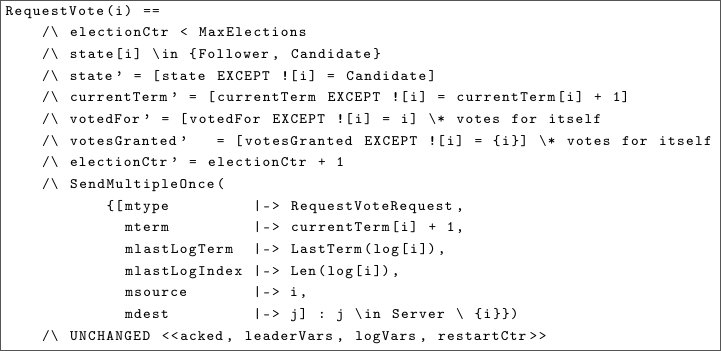
\includegraphics[scale=0.4]{inc/tla-06-request-vote.png}
  \caption{Действие $RequestVote$}
  \label{fig:tla-06-request-vote}
\end{figure}

\textbf{2. AppendEntries}

Код действия $AppendEntries$ приведён на
рис.~\ref{fig:tla-06-append-entries}.

\begin{figure}
  \centering
  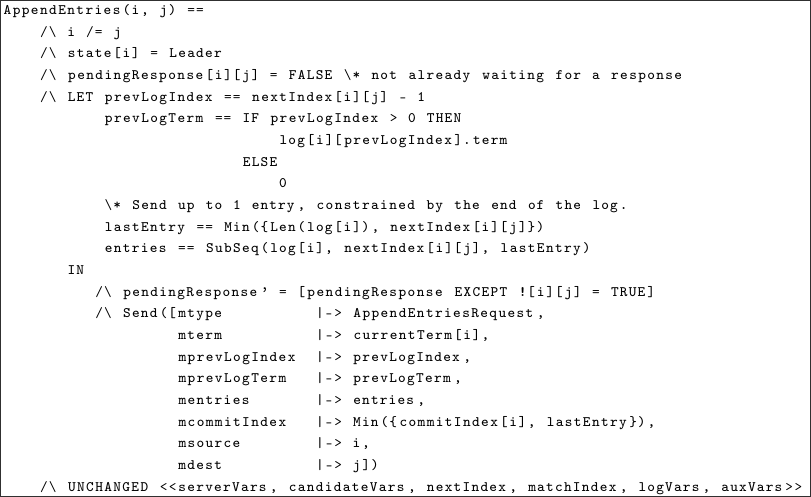
\includegraphics[scale=0.4]{inc/tla-06-append-entries.png}
  \caption{Действие $AppendEntries$}
  \label{fig:tla-06-append-entries}
\end{figure}

Лидер $i$ отправляет серверу $j$ сообщение $AppendEntriesRequest$. В
сообщении передаётся не более одной записи. Условие
$pendingResponse[i][j] = FALSE$ гарантирует, что новый запрос не
отправляется, пока не получен ответ на предыдущий вызов.

\textbf{3. BecomeLeader}

Код действия $BecomeLeader$ приведён на
рис.~\ref{fig:tla-06-become-leader}. Сервер-кандидат $i$ обнаруживает,
что получил кворум голосов, то есть множество $votesGranted[i]$
содержит достаточное число элементов. После этого состояние
$state[i]$ переводится в $Leader$, а переменные $nextIndex[i]$,
$matchIndex[i]$ и $pendingResponse[i]$ инициализируются для начала
репликации журнала.

\begin{figure}
  \centering
  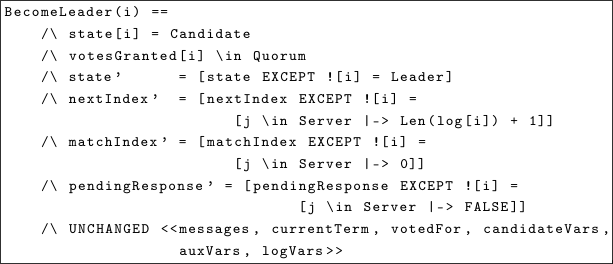
\includegraphics[scale=0.4]{inc/tla-06-become-leader.png}
  \caption{Действие $BecomeLeader$}
  \label{fig:tla-06-become-leader}
\end{figure}

\textbf{4. AdvanceCommitIndex}

Код действия $AdvanceCommitIndex$ приведён на
рис.~\ref{fig:tla-06-advance-commit-index}.

\begin{figure}
  \centering
  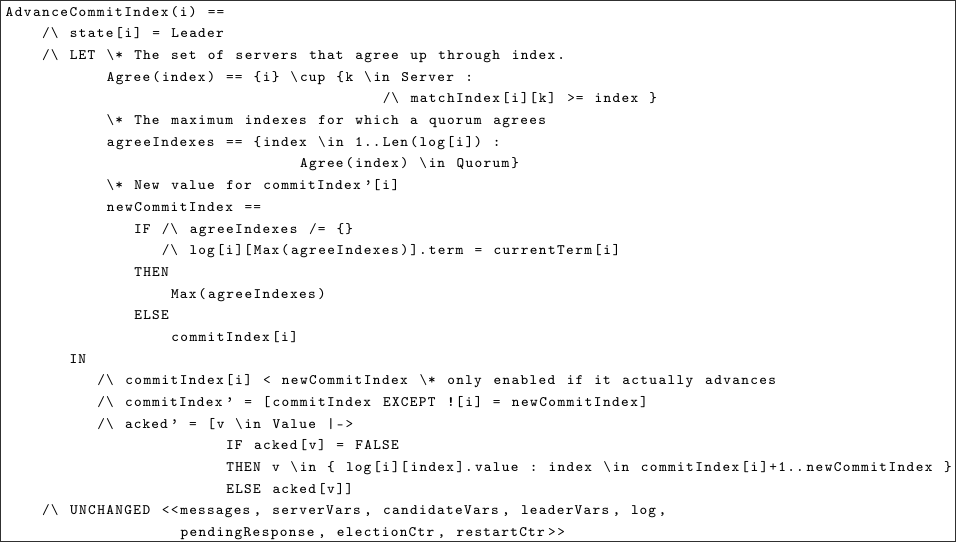
\includegraphics[scale=0.4]{inc/tla-06-advance-commit-index.png}
  \caption{Действие $AdvanceCommitIndex$}
  \label{fig:tla-06-advance-commit-index}
\end{figure}

Лидер $i$ пытается продвинуть индекс фиксации $commitIndex$, если для
некоторого индекса существует подтверждение большинства узлов. Для
этого рассматривается множество серверов, для которых выполнено
условие $matchIndex[i][k] \ge index$, и вычисляется максимальный индекс,
по которому у лидера имеется кворум. Если этот индекс принадлежит
текущему сроку лидера, значение $commitIndex[i]$ обновляется. Все
значения, соответствующие таким новым зафиксированным записям,
помечаются как подтверждённые:
$acked[v] = TRUE$.

\textbf{5. UpdateTerm}

Код действия $UpdateTerm$ приведён на
рис.~\ref{fig:tla-06-update-term}. Если в сети присутствует сообщение
со сроком, превышающим текущий срок сервера, то сервер обновляет своё
значение $currentTerm$, сбрасывает голосование и переходит в состояние
$Follower$.

\begin{figure}
  \centering
  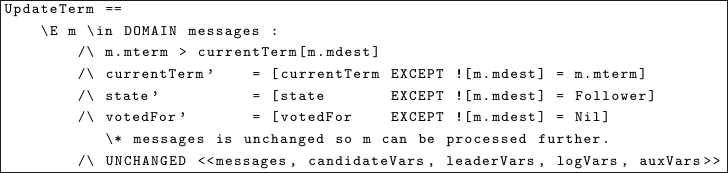
\includegraphics[scale=0.4]{inc/tla-06-update-term.png}
  \caption{Действие $UpdateTerm$}
  \label{fig:tla-06-update-term}
\end{figure}

\textbf{6. HandleRequestVoteRequest}

Код действия $HandleRequestVoteRequest$ приведён на
рис.~\ref{fig:tla-06-handle-request-vote}.

\begin{figure}
  \centering
  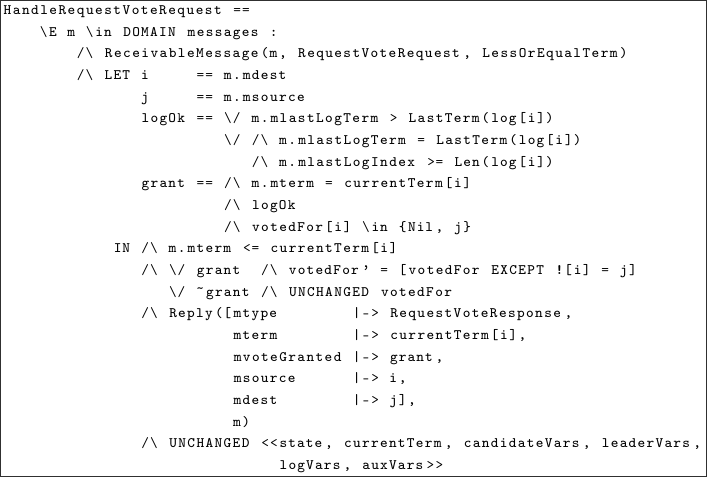
\includegraphics[scale=0.4]{inc/tla-06-handle-request-vote.png}
  \caption{Действие $HandleRequestVoteRequest$}
  \label{fig:tla-06-handle-request-vote}
\end{figure}

Сервер $i$ обрабатывает входящий запрос $RequestVoteRequest$ от
сервера $j$. Сначала проверяется, что срок сообщения не превышает
текущий срок сервера; в противном случае срабатывает действие
$UpdateTerm$. Затем сравнивается состояние журнала кандидата
$(m.mlastLogTerm,\ m.mlastLogIndex)$ с локальным журналом. Если журнал
кандидата не менее актуален, а сервер $i$ ещё не голосовал в данном
сроке либо уже голосовал за $j$, то голос предоставляется. В ответ
отправляется сообщение $RequestVoteResponse$ с полем
$mvoteGranted = grant$.

\textbf{7. HandleRequestVoteResponse}

Код действия $HandleRequestVoteResponse$ приведён на
рис.~\ref{fig:tla-06-handle-request-vote-response}. Сервер $i$
обрабатывает ответ на ранее отправленный запрос голосования. Если
$mvoteGranted = TRUE$, сервер $j$ добавляется в множество
$votesGranted[i]$. После обработки сообщение удаляется из множества
$messages$.

\begin{figure}
  \centering
  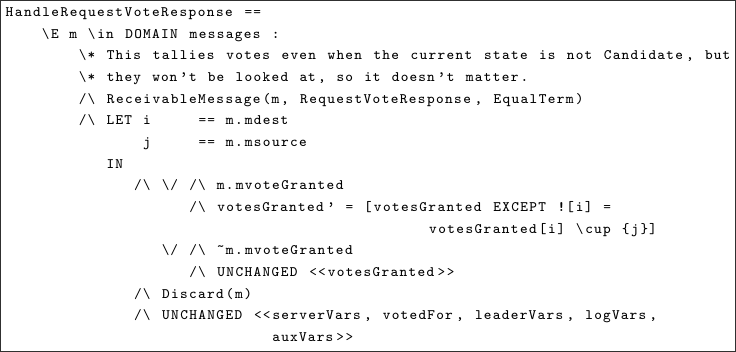
\includegraphics[scale=0.4]{inc/tla-06-handle-request-vote-response.png}
  \caption{Действие $HandleRequestVoteResponse$}
  \label{fig:tla-06-handle-request-vote-response}
\end{figure}

\textbf{8. RejectAppendEntriesRequest}

Код действия $RejectAppendEntriesRequest$ приведён на
рис.~\ref{fig:tla-06-reject-append-entries}. Сервер $i$ отвергает
входящий запрос $AppendEntriesRequest$, если срок сообщения меньше
его собственного либо если сроки совпадают, но журнал получателя не
согласуется с полями $mprevLogTerm$ и $mprevLogIndex$ входящего
сообщения.

\begin{figure}
  \centering
  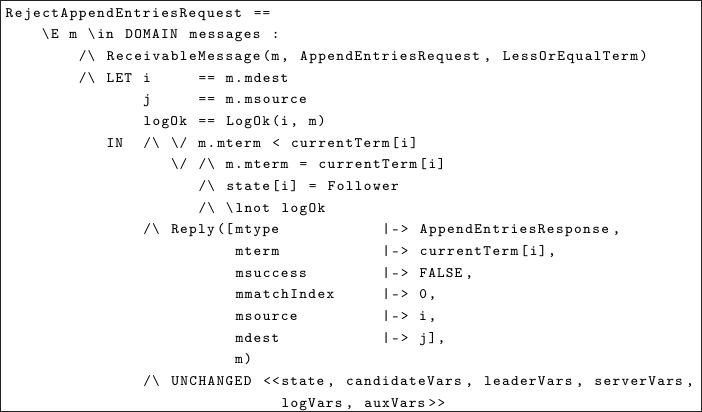
\includegraphics[scale=0.4]{inc/tla-06-reject-append-entries.png}
  \caption{Действие $RejectAppendEntriesRequest$}
  \label{fig:tla-06-reject-append-entries}
\end{figure}

В ответ отправляется сообщение $AppendEntriesResponse$ с полем
$msuccess = FALSE$.

\textbf{9. AcceptAppendEntriesRequest}

Код действия $AcceptAppendEntriesRequest$ приведён на
рис.~\ref{fig:tla-06-accept-append-entries}. В результате его
выполнения может происходить усечение локального журнала и добавление
новой записи. Значение $commitIndex'[i]$ обновляется в соответствии с
информацией, полученной от лидера, что отражает следование
последователя за зафиксированным состоянием лидера. В ответ
отправляется сообщение $AppendEntriesResponse$ с полем
$msuccess = TRUE$.

\begin{figure}
  \centering
  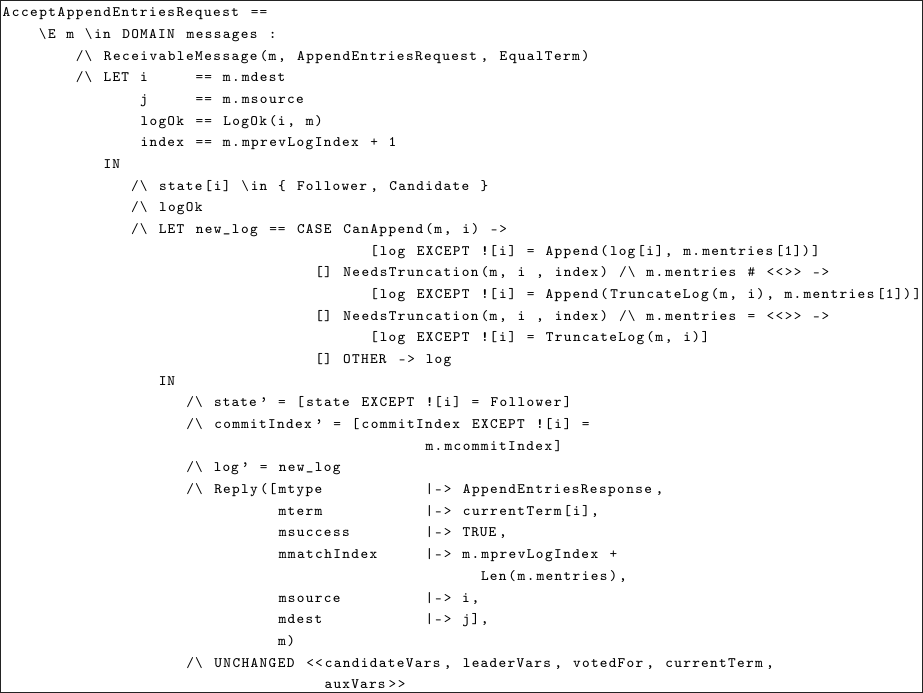
\includegraphics[scale=0.4]{inc/tla-06-accept-append-entries.png}
  \caption{Действие $AcceptAppendEntriesRequest$}
  \label{fig:tla-06-accept-append-entries}
\end{figure}

\textbf{10. HandleAppendEntriesResponse}

Код действия $HandleAppendEntriesResponse$ приведён на
рис.~\ref{fig:tla-06-handle-append-entries-response}.

\begin{figure}
  \centering
  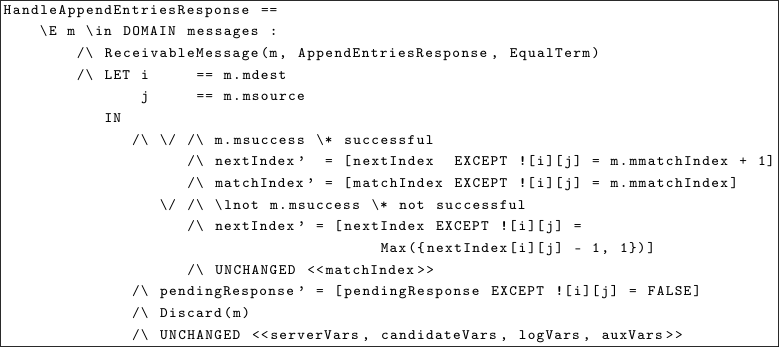
\includegraphics[scale=0.4]{inc/tla-06-handle-append-entries-response.png}
  \caption{Действие $HandleAppendEntriesResponse$}
  \label{fig:tla-06-handle-append-entries-response}
\end{figure}

Лидер $i$ обрабатывает ответ от сервера $j$. Если
$msuccess = TRUE$, то лидер обновляет значения
$matchIndex[i][j]$ и $nextIndex[i][j]$ в соответствии с подтверждённым
состоянием журнала последователя. Если $msuccess = FALSE$, то
$nextIndex[i][j]$ уменьшается на единицу, чтобы повторить попытку
репликации с более ранней позиции. После этого
$pendingResponse'[i][j] = FALSE$, а обработанное сообщение удаляется из
множества сообщений.

Код оператора $Next$ и спецификации приведён на рис.~\ref{fig:tla-07}.

\begin{figure}
  \centering
  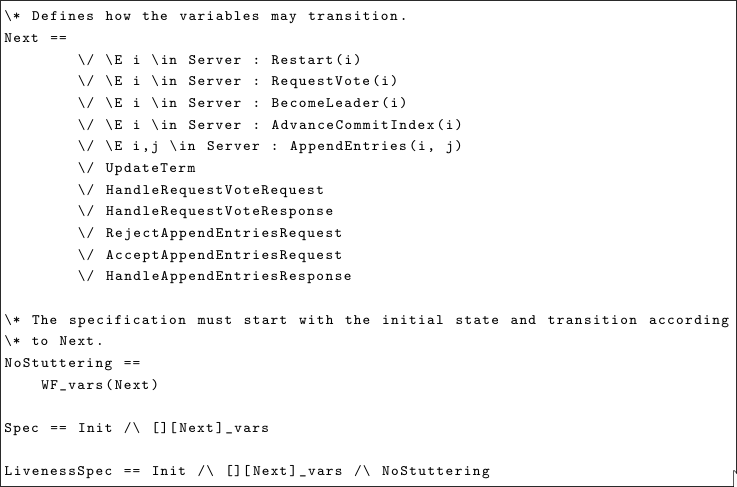
\includegraphics[scale=0.4]{inc/tla-07.png}
  \caption{Спецификация и оператор $Next$}
  \label{fig:tla-07}
\end{figure}

Оператор $Next$ представляет собой дизъюнкцию всех возможных действий,
которые могут быть выполнены системой на одном шаге. В каждый момент
времени система может выполнить одно из перечисленных действий
($Restart$, $RequestVote$, $AppendEntries$, $BecomeLeader$ и другие),
если выполняются соответствующие предусловия.

$Spec$ имеет стандартную для TLA+ структуру: оператор $Init$ задаёт
начальное состояние, а формула $[][Next]_{vars}$ определяет, что на
каждом шаге выполняется одно из действий, входящих в $Next$.

\subsection{Тестирование модели}

Инварианты приведены на рис.~\ref{fig:tla-08}. Они проверяются при
модельной проверке, чтобы убедиться, что основные свойства безопасности
Raft не нарушаются ни при одной последовательности допустимых действий.

\begin{figure}
  \centering
  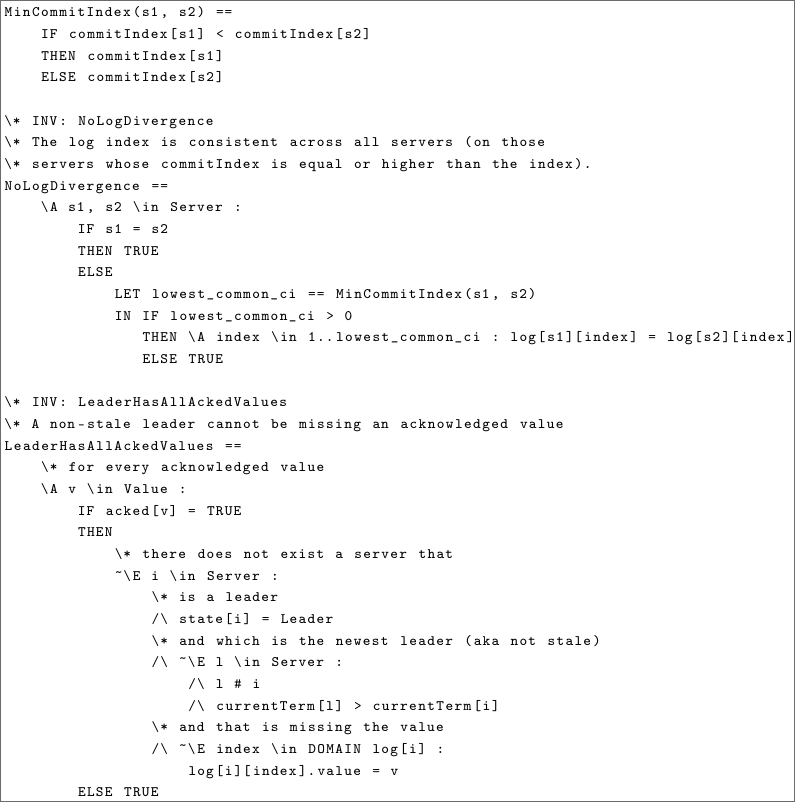
\includegraphics[scale=0.4]{inc/tla-08.png}
  \caption{Инварианты}
  \label{fig:tla-08}
\end{figure}

$NoLogDivergence$ выражает условие, что если у двух серверов некоторый
индекс считается зафиксированным, то записи по этому индексу должны
совпадать. Это одно из ключевых свойств согласованности журнала в
алгоритме Raft.

$LeaderHasAllAckedValues$ задаёт условие, что если некоторое значение
$acked[v] = TRUE$, то любой лидер обязан содержать это значение в своём
журнале.

Разработанная TLA+ спецификация проверялась с помощью средства TLC,
которое перебирает возможные пути выполнения модели и контролирует
выполнение заданных инвариантов.

Конфигурация модели TLC, включающая значения констант, проверяемые
варианты поведения, а также определение начального состояния и
переходного отношения, приведена в приложении.

Результаты проверки приведены на рис.~\ref{fig:tla-09}. В рамках
выбранной конфигурации модели было исследовано более 36 тысяч
состояний. Нарушений заданных инвариантов обнаружено не было.

\begin{figure}
  \centering
  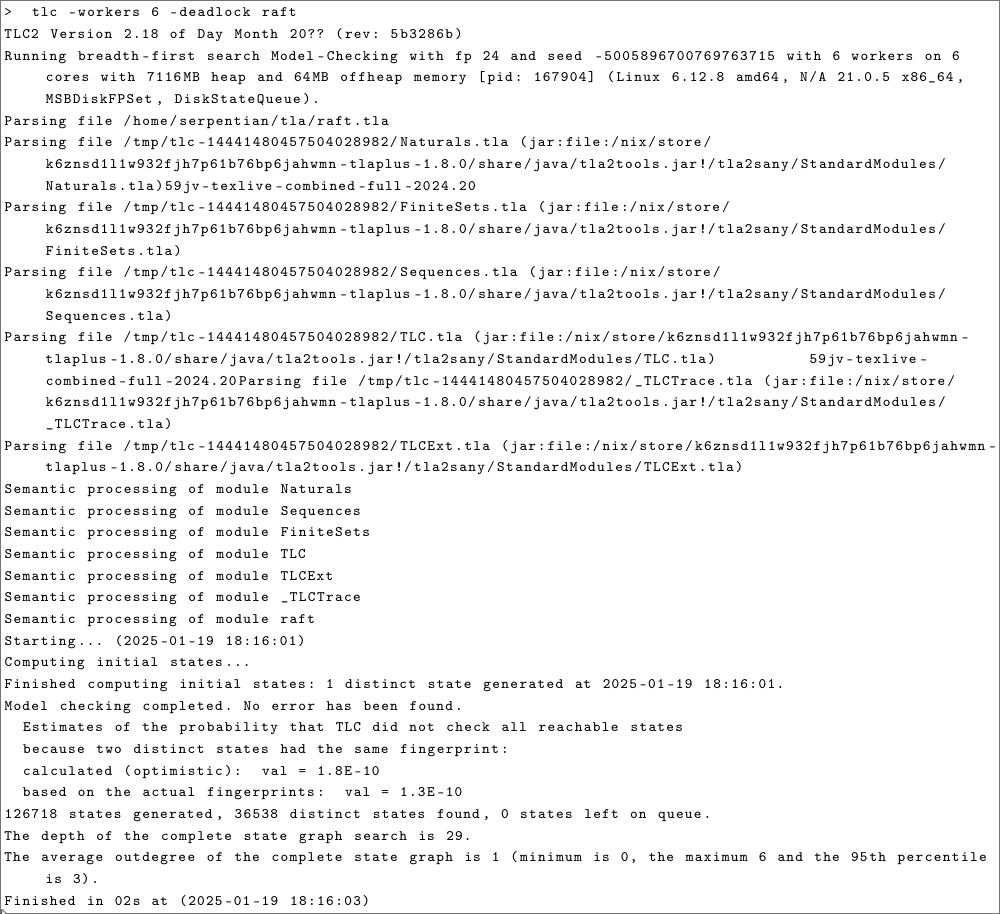
\includegraphics[scale=0.4]{inc/tla-09.png}
  \caption{Проверка модели}
  \label{fig:tla-09}
\end{figure}
